\section{Evaluation}
\label{sec:evaluation}

\subsection{Overall Evaluation Setup}
We evaluate MemT-1.0 from the perspectives of memory and general capabilities.
The memory evaluation focuses on whether MemT-1.0 can answer questions based on its dynamic memory states, without access to prior textual context.
The evaluation on general capabilities examines the impact of the additional native memory mechanism on the model’s general capabilities.
These aspects provide an important foundation for self-evolving memory-native models.

\textbf{Benchmarks.}
We evaluate memory capabilities on 11 benchmarks and divide them into four groups according to trajectory length.
Specifically, the group below 16K includes MemBench~\cite{tan2025membench} and ImplicitMemBench~\cite{qin2026implicitmembench}, and the 16K-32K group includes PersonaMem~\cite{jiang2025know}, PS-Bench~\cite{guo2026personalization}, and LoCoMo~\cite{maharana2024evaluating}.
For longer trajectories, the 32K-64K group includes PerMemSafe~\cite{an2026permemsafe}, Memora~\cite{uddin2026recall}, and MemOps~\cite{hao2026memops}, and the group above 64K includes LongMemEval-S~\cite{wu2024longmemeval}, MemoryAgentBench~\cite{hu2026evaluating}, and BEAM-1M~\cite{tavakoli2025beyond}.
These benchmarks focus on long-term information retention and retrieval, dynamic memory updating and management, and personalized understanding.
In addition, we evaluate general capabilities on six benchmarks spanning four major dimensions.
Specifically, we evaluate knowledge and scientific reasoning with MMLU-Pro~\cite{wang2024mmlu} and GPQA Diamond~\cite{rein2023gpqa}, instruction following with IFEval~\cite{zhou2023instruction},
long-context understanding with LongBench v2~\cite{bai2025longbench}, and code generation with BigCodeBench-Hard~\cite{zhuo2025bigcodebench} and LiveCodeBench v6~\cite{jain2025livecodebench}.
These benchmarks collectively assess a wide range of general capabilities, thereby reflecting the impact of the additional native memory mechanism on the underlying backbone model.
More details are available in Appendix~\ref{appendix:benchmark_details}.

\textbf{Baselines.}
We compare MemT-1.0 with textual memory and parametric memory approaches.
Textual memory methods perform inference based on the original backbone model with full context and partial context settings.
Full context provides the complete historical text as memory in the input context, while DenseRAG retrieves a subset of relevant information as contextual evidence~\cite{karpukhin2020densepassageretrievalopendomain}.
We also include representative memory systems for comparison, including MemOS~\cite{li2025memos}, Mem0~\cite{chhikara2025mem0}, OpenViking~\cite{fu2026vikingmem}, and Graphiti~\cite{rasmussen2025zep}.
For parametric memory methods, no textual history is provided in the context, and the model performs inference using its own parametric memory.
Our parametric memory baselines include Temp-LoRA~\cite{wang2024greater}, Doc-to-LoRA~\cite{charakorn2026doc}, SHINE~\cite{liu2026shine}, $\delta$-mem~\cite{lei2026delta}, LiveMem~\cite{liu2026livemem}, MemoryLLM~\cite{wang2024memoryllm} and ICAE~\cite{ge2023context}.
More details of the baselines are provided in Appendix~\ref{appendix:baseline_details}.

\textbf{Evaluation Protocol.}
For memory capability evaluation, in each trajectory, we first reset the memory and write the historical information into memory following the chronological order.
Then, the model is required to answer multiple questions related to the historical information, and the responses are compared against the ground-truth answers to compute accuracy.
Specifically, memory is strictly isolated across different users and histories. 
Ground-truth answers, evidence annotations, and evaluation labels are only used for scoring and are never exposed to the evaluated models.
For LLM-as-a-Judge, we utilize \texttt{gpt-4.1-mini} with the OmniMemEval~\cite{memtensor2026omnimemeval} prompt.
For general capability evaluation, we introduce irrelevant information before inference, which aims to examine how the native memory mechanism affects the model’s general capabilities under the noise setting.
More details are available in Appendix~\ref{appendix:eval_general_pipeline_details}.

\begin{table*}[!t]
    \centering
    \caption{Memory capability evaluation across 11 benchmarks.
        Benchmarks are grouped according to trajectory length.
        DS indicates DeepSeek-V4-Flash, while QW means Qwen3.6-35B-A3B.
        Bold and underlined values indicate the best and second-best
        results within each memory category, respectively.
    }
    \label{tab:memory_capability_main}

    \begin{threeparttable}

    \renewcommand{\arraystretch}{1.16}

    \sisetup{
        detect-weight = true,
        detect-family = true,
        round-mode = figures,
        round-precision = 3,
        round-pad = true,
        table-alignment-mode = none,
        table-number-alignment = center,
        table-text-alignment = center
    }

    \newcommand{\best}[1]{{\bfseries\num{#1}}}
    \newcommand{\secondbest}[1]{\underline{\num{#1}}}

    \newcolumntype{Y}{
        S[
            table-fixed-width = true,
            table-column-width = 2.0 em,
            table-alignment-mode = none,
            table-number-alignment = center,
            table-text-alignment = center
        ]
    }

    \begin{adjustbox}{max width=\textwidth}
    \begin{tabular}{
        l
        c
        Y Y Y Y Y Y Y Y Y Y Y Y
    }

    \toprule[1.15pt]

    \rowcolor{MetisBlueDark}
    \color{white}\bfseries Method
    &
    \color{white}\bfseries Backbone
    &
    \multicolumn{2}{c}{\color{white}\bfseries $<16$K}
    &
    \multicolumn{3}{c}{\color{white}\bfseries 16--32K}
    &
    \multicolumn{3}{c}{\color{white}\bfseries 32--64K}
    &
    \multicolumn{3}{c}{\color{white}\bfseries $>64$K}
    &
    \multicolumn{1}{c}{\color{white}\bfseries All}
    \\

    \rowcolor{MetisBlueLight}
    &
    &
    \multicolumn{1}{c}{\bfseries MB}
    &
    \multicolumn{1}{c}{\bfseries IM}
    &
    \multicolumn{1}{c}{\bfseries PM}
    &
    \multicolumn{1}{c}{\bfseries PSB}
    &
    \multicolumn{1}{c}{\bfseries LCM}
    &
    \multicolumn{1}{c}{\bfseries PMS}
    &
    \multicolumn{1}{c}{\bfseries MMR}
    &
    \multicolumn{1}{c}{\bfseries MO}
    &
    \multicolumn{1}{c}{\bfseries LME}
    &
    \multicolumn{1}{c}{\bfseries MAB}
    &
    \multicolumn{1}{c}{\bfseries BEAM}
    &
    \multicolumn{1}{c}{\bfseries AVG}
    \\

    \midrule[0.65pt]

    \rowcolor{MetisBluePale}
    \multicolumn{14}{c}{
        \textcolor{MetisBlueDark}{\bfseries Textual Memory}
    }
    \\

    \addlinespace[1pt]

    \multirow{2}{*}{MemOS}
    & DS
    & 78.38 & {\best{68.15}}
    & 67.06 & 92.86 & {\best{85.65}}
    & 45.87 & {\best{55.52}} & 76.95
    & {\best{83.20}} & 27.78 & {\best{72.59}}
    & {\best{68.55}}
    \\

    & QW
    & 79.87 & {\secondbest{61.14}}
    & {\best{67.57}} & 97.32 & 83.38
    & 54.67 & 52.61 & 82.56
    & 80.80 & 21.78 & 71.31
    & {\secondbest{68.46}}
    \\

    \addlinespace[2pt]

    \multirow{2}{*}{Mem0}
    & DS
    & 75.79 & 45.85
    & {\secondbest{67.23}} & 89.43 & 78.96
    & {\best{66.00}} & 47.52 & 75.67
    & 72.60 & 30.30 & 71.43
    & 65.53
    \\

    & QW
    & 78.52 & 60.41
    & 63.16 & 97.32 & 80.91
    & 54.93 & 41.40 & 79.42
    & 78.90 & 20.56 & 70.27
    & 65.98
    \\

    \addlinespace[2pt]

    \multirow{2}{*}{OpenViking}
    & DS
    & 75.72 & 41.39
    & 65.37 & 95.44 & 79.09
    & 53.20 & {\secondbest{53.43}} & 77.27
    & 75.00 & 28.15 & {\secondbest{71.92}}
    & 65.09
    \\

    & QW
    & 76.77 & 53.03
    & 61.63 & 95.92 & 72.92
    & 53.73 & 51.45 & 81.74
    & {\secondbest{82.00}} & 23.20 & 67.32
    & 65.43
    \\

    \addlinespace[2pt]

    \multirow{2}{*}{Graphiti}
    & DS
    & 49.58 & 39.41
    & 53.65 & 89.00 & 66.69
    & 30.80 & 26.22 & 51.08
    & 57.00 & 19.85 & 60.44
    & 49.43
    \\

    & QW
    & 61.93 & 34.94
    & 49.75 & 96.51 & 50.58
    & 24.53 & 23.04 & 47.43
    & 38.10 & 15.52 & 60.59
    & 45.72
    \\

    \addlinespace[2pt]

    \multirow{2}{*}{Full Context}
    & DS
    & {\secondbest{83.23}} & 58.04
    & 65.20 & 97.37 & 79.87
    & 32.27 & 51.65 & {\secondbest{88.72}}
    & 77.80 & {\best{35.98}} & 44.65
    & 64.98
    \\

    & QW
    & {\best{84.32}} & 53.63
    & 65.20 & {\best{98.66}} & {\secondbest{83.77}}
    & 44.80 & 49.79 & {\best{92.40}}
    & 76.80 & {\secondbest{35.94}} & 43.66
    & 66.27
    \\

    \addlinespace[2pt]

    \multirow{2}{*}{DenseRAG}
    & DS
    & 69.30 & 55.03
    & 59.42 & 89.05 & 58.31
    & {\secondbest{55.47}} & 31.40 & 68.53
    & 69.40 & 30.48 & 43.71
    & 57.28
    \\

    & QW
    & 67.09 & 52.15
    & 60.27 & {\secondbest{97.69}} & 61.10
    & 45.20 & 31.28 & 70.55
    & 70.80 & 28.17 & 37.09
    & 56.49
    \\

    \addlinespace[2pt]
    \midrule[0.5pt]

    \rowcolor{MetisBluePale}
    \multicolumn{14}{c}{
        \textcolor{MetisBlueDark}{\bfseries Parametric Memory}
    }
    \\

    \addlinespace[1pt]

    \rowcolor{MetisHighlightStrong}
    \textcolor{MetisBlueDark}{\bfseries MemT-1.0-Flash}
    & --
    & {\best{73.48}} & {\best{49.21}}
    & {\best{61.63}} & {\secondbest{97.48}} & {\best{65.13}}
    & 33.47 & {\secondbest{20.54}} & {\best{64.06}}
    & {\best{37.20}} & {\best{17.36}} & {\best{37.04}}
    & {\best{50.60}}
    \\

    \rowcolor{MetisHighlight}
    \textcolor{MetisBlueDark}{\bfseries MemT-1.0-Nano}
    & --
    & {\secondbest{71.75}} & {\secondbest{43.11}}
    & 52.29 & {\num{95.71}} & {\secondbest{57.53}}
    & {\best{38.67}} & {\best{23.92}} & 49.85
    & {\secondbest{32.60}} & {\secondbest{15.48}} & {\secondbest{35.78}}
    & {\secondbest{46.97}}
    \\

    \addlinespace[2pt]

    Temp-LoRA
    & --
    & {\num{44.25}} & 32.03
    & {\secondbest{57.39}} & {\best{98.01}} & 25.13
    & {\secondbest{35.73}} & 16.17 & {\secondbest{52.50}}
    & 13.40 & 11.98 & 32.32
    & 38.08
    \\

    Doc-to-LoRA
    & --
    & 57.19 & 42.42
    & 33.96 & 70.21 & 24.48
    & 16.53 & 15.31 & 36.01
    & 14.60 & 3.54 & 25.99
    & 30.93
    \\

    SHINE
    & --
    & 40.70 & 20.24
    & 39.90 & 63.29 & 26.69
    & 4.40 & 16.74 & 39.59
    & 13.80 & 6.15 & 9.58
    & 25.55
    \\

    $\delta$-mem
    & --
    & 37.48 & 29.92
    & 46.86 & 90.82 & 20.26
    & 20.13 & 17.89 & 40.92
    & 14.80 & 7.13 & 17.03
    & 31.20
    \\

    LiveMem-RL
    & --
    & 35.67 & 23.31
    & 46.01 & 82.02 & 24.42
    & 10.53 & 16.37 & 39.83
    & 14.60 & 7.27 & 27.08
    & 29.74
    \\

    MemoryLLM
    & --
    & 22.71 & 17.76
    & 41.09 & 37.41 & 46.62
    & 3.33 & 16.26 & 46.80
    & 15.60 & 6.26 & 24.01
    & 25.26
    \\

    ICAE
    & --
    & 31.90 & 24.49
    & 17.83 & 70.37 & 22.40
    & 2.80 & 11.35 & 40.41
    & 11.00 & 7.35 & 11.69
    & 22.87
    \\

    \bottomrule[1.15pt]

    \end{tabular}
    \end{adjustbox}

    \vspace{2pt}

    \begin{minipage}{\textwidth}
        \footnotesize
        \textit{Abbreviations.}
        \textbf{MB}: MemBench;
        \textbf{IM}: ImplicitMemBench;
        \textbf{PM}: PersonaMem;
        \textbf{PSB}: PS-Bench;
        \textbf{LCM}: LoCoMo;
        \textbf{PMS}: PerMemSafe;
        \textbf{MMR}: Memora;
        \textbf{MO}: MemOps;
        \textbf{LME}: LongMemEval-S;
        \textbf{MAB}: MemoryAgentBench;
        \textbf{BEAM}: BEAM-1M.
    \end{minipage}

    \end{threeparttable}
    \vspace{-0.4cm}
\end{table*}

\subsection{Memory Capabilities}
The results for memory capabilities are presented in Table~\ref{tab:memory_capability_main}.
MemT-1.0-Flash and MemT-1.0-Nano achieve average scores of 50.6 and 47.0, respectively, ranking first and second among the parametric memory methods, ahead of the strongest parametric baseline by 12.5 and 8.9 points.
The results support native memory as a shared representation for diverse memory tasks without providing historical text in the query context.
The comparison between MemT-1.0-Flash and MemT-1.0-Nano reveals distinct strengths across tasks, though the aggregate gap between them remains modest and is driven mainly by memory operations.
MemT-1.0-Flash improves most clearly on memory operations, personalized understanding, conversational recall, and implicit learning.
MemT-1.0-Nano remains stronger on PerMemSafe and Memora, whereas MemT-1.0-Flash scores higher on Persona-grounded PS-Bench.
The advantage over parametric memory baselines also extends to long histories, where MemT-1.0 leads this group on LongMemEval-S, MemoryAgentBench, and BEAM-1M.
However, the remaining errors on these benchmarks show that processing an extended trajectory does not by itself ensure reliable access to its contents.
Answering later queries requires earlier information to survive successive updates and remain distinguishable from other stored associations.
The results motivate further improvements in selective retention and query-dependent readout.

The strongest textual memory systems still achieve substantially higher performance, particularly on LongMemEval-S and BEAM-1M.
These systems provide explicit historical evidence at query time, whereas MemT-1.0 must recover the required information from its evolving states.
This gap is consistent with the difficulty of preserving detailed evidence through recurrent memory updates and highlights memory fidelity as an important target for further development.

\subsection{General Capabilities}
We evaluate general capabilities under the noise setting.
In this setting, we inject irrelevant information into memory before the evaluation tasks, which simulates the impact of distracting memories during real-world online interactions.
We report the performance gap between MemT-1.0 and its corresponding backbone model under the noise setting.
The results are presented in Table~\ref{tab:general_capability}.

MemT-1.0-Flash performs comparably to its DeepSeek-V4-Flash backbone on average under the same noise setting.
The largest gain occurs on BigCodeBench-Hard, with smaller improvements on IFEval and LongBench v2.
Performance decreases modestly on MMLU-Pro, GPQA Diamond, and LiveCodeBench v6.
These results suggest that MemT-1.0-Flash broadly preserves general capabilities under distracting memories.

We next examine MemT-1.0-Nano, whose average decrease is around one point.
Under the noise setting, most benchmarks remain close to the backbone, with gains on IFEval and BigCodeBench-Hard.
The degradation is concentrated rather than uniform.
The largest decrease occurs on LiveCodeBench v6, followed by smaller decreases on LongBench v2, MMLU-Pro, and GPQA Diamond.
The contrasting changes on BigCodeBench-Hard and LiveCodeBench v6 further suggest that the impact varies even across benchmarks within the same capability domain.

Overall, the results support broad capability preservation alongside native memory, while highlighting that resistance to distracting memories should be evaluated at the task level.

\begin{table*}[t]
    \centering
    \caption{
        General capability evaluation under the backbone and noise settings.
        MemT-1.0 results report score differences relative to the
        corresponding backbone under the same setting.
    }
    \label{tab:general_capability}

    \begin{threeparttable}

    \renewcommand{\arraystretch}{1.16}

    \sisetup{
        round-mode = places,
        round-precision = 1,
        round-pad = true,
        table-number-alignment = center
    }

    \newcommand{\gcDown}[1]{%
        \multicolumn{1}{c}{%
            \textcolor{MetisDeltaDown}{\ensuremath{-#1}}%
        }%
    }
    \newcommand{\gcUp}[1]{%
        \multicolumn{1}{c}{%
            \textcolor{MetisDeltaUp}{\ensuremath{+#1}}%
        }%
    }
    \newcommand{\gcNA}{\multicolumn{1}{c}{--}}
    \newcommand{\gcZero}{\multicolumn{1}{c}{0.0}}

    \begin{adjustbox}{max width=\textwidth}
    \begin{tabular}{
        l
        *{7}{S[
            table-format = 2.1,
            table-fixed-width = true,
            table-column-width = 4.5 em
        ]}
    }

    \toprule[1.15pt]

    \rowcolor{MetisBlueDark}
    \color{white}\bfseries Model
    & \multicolumn{1}{c}{\color{white}\bfseries MP}
    & \multicolumn{1}{c}{\color{white}\bfseries GPQA}
    & \multicolumn{1}{c}{\color{white}\bfseries IFE}
    & \multicolumn{1}{c}{\color{white}\bfseries LB}
    & \multicolumn{1}{c}{\color{white}\bfseries BCB-H}
    & \multicolumn{1}{c}{\color{white}\bfseries LCB-v6}
    & \multicolumn{1}{c}{\color{white}\bfseries AVG}
    \\

    \midrule[0.65pt]

    \rowcolor{MetisBluePale}
    \multicolumn{8}{c}{
        \textcolor{MetisBlueDark}{\bfseries Backbone}
    }
    \\

    \addlinespace[1pt]

    DeepSeek-V4-Flash
    & 85.68
    & 91.16
    & 93.53
    & 63.02
    & 35.81
    & 87.49
    & 76.12
    \\

    Qwen3.6-35B-A3B
    & 84.58
    & 83.90
    & 90.57
    & 57.26
    & 27.03
    & 87.96
    & 71.88
    \\

    \addlinespace[2pt]
    \midrule[0.5pt]

    \rowcolor{MetisBluePale}
    \multicolumn{8}{c}{
        \textcolor{MetisBlueDark}{\bfseries Noise Setting}
    }
    \\

    \addlinespace[1pt]

    DeepSeek-V4-Flash
    & 83.81
    & 89.58
    & 92.98
    & 64.21
    & 32.43
    & 89.19
    & 75.37
    \\

    \rowcolor{MetisHighlightStrong}
    \textcolor{MetisBlueDark}{\bfseries MemT-1.0-Flash}
    & \gcDown{1.8}
    & \gcDown{0.6}
    & \gcUp{0.9}
    & \gcUp{0.2}
    & \gcUp{2.0}
    & \gcDown{0.7}
    & \gcZero
    \\

    Qwen3.6-35B-A3B
    & 84.42
    & 80.05
    & 89.28
    & 55.67
    & 25.68
    & 88.06
    & 70.53
    \\

    \rowcolor{MetisHighlight}
    \textcolor{MetisBlueDark}{\bfseries MemT-1.0-Nano}
    & \gcDown{1.6}
    & \gcDown{1.5}
    & \gcUp{3.3}
    & \gcDown{2.0}
    & \gcUp{2.0}
    & \gcDown{5.8}
    & \gcDown{0.9}
    \\

    \bottomrule[1.15pt]

    \end{tabular}
    \end{adjustbox}

    \vspace{2pt}

    \begin{minipage}{\textwidth}
        \footnotesize
        \textit{Abbreviations.}
        \textbf{MP}: MMLU-Pro;
        \textbf{GPQA}: GPQA Diamond;
        \textbf{IFE}: IFEval;
        \textbf{LB}: LongBench v2;
        \textbf{BCB-H}: BigCodeBench-Hard;
        \textbf{LCB-v6}: LiveCodeBench v6.
        AVG is the unweighted average across the six benchmarks.
        For MemT-1.0, values denote score-point differences
        relative to the corresponding backbone under the noise setting.
        \textcolor{MetisDeltaDown}{Green} indicates a decrease,
        while \textcolor{MetisDeltaUp}{red} indicates an increase.
    \end{minipage}

    \end{threeparttable}
    \vspace{-0.4cm}
\end{table*}

\subsection{Ablation Studies}
In this section, we further present several ablation studies based on MemT-1.0-Nano during model development.
As for the model architecture, we focus on the update rule and update granularity in the native memory procedure.
We also design a bidirectional encoding mechanism to aggregate information from the current turn.
In addition, we study the contribution of different training stages.
These experiments further verify the effectiveness of our current architecture.

\subsubsection{Architecture Ablation}

For architecture ablation, we evaluate four variants.
First, we remove the stable mechanism to recover the GDN-2 memory update (w/ GDN-2) by directly using
\begin{equation*}
    \tilde{\mathbf{M}}_{t, i, h}^{(l)} = \left[
\mathbf{I}
-
\mathbf{K}_{t,i,h}^{(l)\top}
\left(
\bm{\beta}_{t,i,h}^{(l)}
\odot
\mathbf{K}_{t,i,h}^{(l)}
\right)
\right]
\cdot
\mathbf{D}_{t,i,h}^{(l)}
\tilde{\mathbf{M}}_{t,i-1,h}^{(l)}
+
\mathbf{K}_{t,i,h}^{(l)\top}
\left(
\bm{\omega}_{t,i,h}^{(l)}
\odot
\mathbf{V}_{t,i,h}^{(l)}
\right).
\end{equation*}
We also change the update rule into GDN~\cite{yang2025gateddeltanetworksimproving} as another ablation baseline (w/ GDN).
Second, we change the update granularity from token-level to turn-level (w/ TL).
The storage procedure can be defined as
\begin{equation*}
    \mathbf{M}_{t+1,h}^{(l)} = \left[
\mathbf{I}
-
\frac{1}{L_t}
\mathbf{U}_{t,h}^{(l)\top}
\mathbf{U}_{t,h}^{(l)}
\right]
\cdot
\mathbf{D}_{t,h}^{(l)}
\mathbf{M}_{t,h}^{(l)}
+
\frac{1}{L_t}
\mathbf{U}_{t,h}^{(l)\top}
\left(
\bm{\omega}_{t,h}^{(l)}
\odot
\mathbf{V}_{t,h}^{(l)}
\right),
\end{equation*}
where we have 
\begin{equation*}
    \mathbf{D}_{t,h}^{(l)} = \operatorname{Diag}
\left[
\exp
\left(
\frac{1}{L_t}
\sum_{i=1}^{L_t}
\bm{\lambda}_{t,i,h}^{(l)}
\right)
\right].
\end{equation*}
We also evaluate a bidirectional encoding (w/ BE) for information aggregation.
Specifically, during the storage procedure in each turn, it first projects the pre-attention hidden states $\tilde{\mathbf{H}}_t^{(l)}$ into a lower-dimensional space, and applies multi-head self-attention with rotary position embeddings without a causal mask.
After that, it projects the result back to the backbone dimension through a residual connection.
The enriched representations are used to predict the erase, write, and forget gates, while the memory keys and values are still projected from the original pre-attention hidden states.

As shown in Table~\ref{tab:ablation_results}, the update granularity has the largest effect among the architecture variants.
Replacing token-level with turn-level aggregation reduces the average from 46.97 to 40.98, a far larger drop than any change to the update rule.
This may be because successive token-level updates can better account for memory decay and revise associations established earlier within the same turn.
The update-rule variants, by contrast, stay close to the full model, with removing the stable mechanism giving 46.43 and substituting GDN giving 46.72.
Both fall within a narrow band around the baseline, so the aggregate capability is not determined by the precise form of the update rule.
Adding bidirectional encoding reduces the average to 45.43.
Its effect is benchmark-dependent rather than uniformly negative: MB, IM, PM, and PMS improve, whereas the remaining benchmarks regress.
Under the evaluated training budget, bidirectional encoding does not improve aggregate memory performance, and its benchmark-specific gains do not offset the losses elsewhere.

\subsubsection{Training Ablation}
We further conduct ablation studies on our training procedures.
For the w/o CPT setting, we skip CPT and directly train the memory parameters through post-training alone.
For the w/o PT setting, we evaluate the checkpoint after continued pre-training without subsequent post-training.
From the results in Table~\ref{tab:ablation_results}, we find that post-training plays an important role in memory-specific tasks, where it increases the average score by approximately 10.69 points over the CPT checkpoint.
These results indicate that language-modeling CPT alone does not provide the same memory-conditioned response capability as the complete pipeline.
In addition, the CPT stage improves post-training as well.
Therefore, post-training accounts for the larger observed gain in this comparison, while CPT provides an additional aggregate benefit as an initialization stage.

\begin{table*}[t]
    \centering
    \caption{
        Architecture and training ablations of MemT-1.0-Nano.
        Bold and underlined values indicate the best and
        second-best results, respectively.
        $\Delta$ AVG denotes the score difference relative
        to MemT-1.0-Nano.
    }
    \label{tab:ablation_results}

    \begin{threeparttable}

    \setlength{\tabcolsep}{3.2pt}
    \renewcommand{\arraystretch}{1.16}

    \sisetup{
        detect-weight = true,
        detect-family = true,
        round-mode = places,
        round-precision = 1,
        round-pad = true,
        table-alignment-mode = none,
        table-number-alignment = center,
        table-text-alignment = center
    }

    \newcommand{\abfirst}[1]{{\bfseries\num{#1}}}
    \newcommand{\absecond}[1]{{\underline{\num{#1}}}}

    \newcolumntype{Y}{
        S[
            table-fixed-width = true,
            table-column-width = 2.8em,
            table-alignment-mode = none,
            table-number-alignment = center,
            table-text-alignment = center
        ]
    }

    \newcolumntype{Z}{
        S[
            table-fixed-width = true,
            table-column-width = 3.8em,
            table-alignment-mode = none,
            table-number-alignment = center,
            table-text-alignment = center
        ]
    }

    \begin{adjustbox}{max width=\textwidth}
    \begin{tabular}{
        l
        Y Y Y Y Y Y Y Y Y Y Y Y Z
    }

    \toprule[1.15pt]

    \rowcolor{MetisBlueDark}
    \color{white}\bfseries Variant
    &
    \multicolumn{2}{c}{\color{white}\bfseries $<16$K}
    &
    \multicolumn{3}{c}{\color{white}\bfseries 16--32K}
    &
    \multicolumn{3}{c}{\color{white}\bfseries 32--64K}
    &
    \multicolumn{3}{c}{\color{white}\bfseries $>64$K}
    &
    \multicolumn{2}{c}{\color{white}\bfseries All}
    \\

    \rowcolor{MetisBlueLight}
    &
    \multicolumn{1}{c}{\bfseries MB}
    &
    \multicolumn{1}{c}{\bfseries IM}
    &
    \multicolumn{1}{c}{\bfseries PM}
    &
    \multicolumn{1}{c}{\bfseries PSB}
    &
    \multicolumn{1}{c}{\bfseries LCM}
    &
    \multicolumn{1}{c}{\bfseries PMS}
    &
    \multicolumn{1}{c}{\bfseries MMR}
    &
    \multicolumn{1}{c}{\bfseries MO}
    &
    \multicolumn{1}{c}{\bfseries LME}
    &
    \multicolumn{1}{c}{\bfseries MAB}
    &
    \multicolumn{1}{c}{\bfseries BEAM}
    &
    \multicolumn{1}{c}{\bfseries AVG}
    &
    \multicolumn{1}{c}{\bfseries $\Delta$ AVG}
    \\

    \midrule[0.65pt]

    \rowcolor{MetisHighlight}
    \textcolor{MetisBlueDark}{\bfseries MemT-1.0-Nano}
    & \num{71.75}
    & 43.11
    & 52.29
    & \num{95.71}
    & {\abfirst{57.53}}
    & 38.67
    & {\abfirst{23.92}}
    & 49.85
    & {\abfirst{32.60}}
    & {\abfirst{15.48}}
    & {\abfirst{35.78}}
    & \abfirst{46.97}
    & 0.00
    \\

    \addlinespace[2pt]
    \midrule[0.5pt]

    \rowcolor{MetisBluePale}
    \multicolumn{14}{c}{
        \textcolor{MetisBlueDark}{
            \bfseries Architecture Ablation
        }
    }
    \\

    \addlinespace[1pt]

    w/ GDN-2
    & \num{71.58}
    & {\absecond{43.74}}
    & {\abfirst{55.69}}
    & \num{96.24}
    & 57.34
    & 36.93
    & {\absecond{21.71}}
    & 49.15
    & 29.40
    & 14.38
    & 34.59
    & \num{46.43}
    & \num{-0.54}
    \\

    \addlinespace[2pt]

    w/ GDN
    & \absecond{72.27}
    & 41.92
    & 54.50
    & \abfirst{98.34}
    & {\absecond{57.47}}
    & {\abfirst{40.93}}
    & 20.30
    & {\abfirst{50.60}}
    & {\absecond{30.00}}
    & 13.43
    & 34.15
    & \absecond{46.72}
    & \num{-0.25}
    \\

    \addlinespace[2pt]

    w/ BE
    & \abfirst{73.88}
    & {\abfirst{44.73}}
    & 54.33
    & \num{94.85}
    & 55.39
    & {\absecond{40.80}}
    & 16.27
    & 45.51
    & 25.60
    & {\absecond{14.44}}
    & 33.97
    & \num{45.43}
    & \num{-1.54}
    \\

    \addlinespace[2pt]

    w/ TL
    & \num{69.12}
    & 39.46
    & 52.12
    & \absecond{97.48}
    & 52.86
    & 36.40
    & 17.15
    & 38.29
    & 25.00
    & 5.48
    & 17.39
    & \num{40.98}
    & \num{-5.99}
    \\

    \addlinespace[2pt]
    \midrule[0.5pt]

    \rowcolor{MetisBluePale}
    \multicolumn{14}{c}{
        \textcolor{MetisBlueDark}{
            \bfseries Training Ablation
        }
    }
    \\

    \addlinespace[1pt]

    w/o CPT
    & \num{69.80}
    & 37.42
    & {\absecond{54.67}}
    & \num{96.78}
    & 55.52
    & 35.33
    & 18.68
    & {\absecond{50.15}}
    & 27.00
    & 13.37
    & {\absecond{34.66}}
    & \num{44.85}
    & \num{-2.12}
    \\

    \addlinespace[2pt]

    w/o PT
    & \num{66.19}
    & 38.69
    & 41.26
    & \num{90.23}
    & 40.39
    & 26.27
    & 16.09
    & 24.63
    & 13.80
    & 12.21
    & 29.36
    & \num{36.28}
    & \num{-10.69}
    \\

    \bottomrule[1.15pt]

    \end{tabular}
    \end{adjustbox}

    \end{threeparttable}
    \vspace{-0.4cm}
\end{table*}

\subsection{End-to-End Inference Efficiency}
\label{sec:inference_efficiency}
We further evaluate the end-to-end inference efficiency of MemT-1.0 against baseline methods, with a particular focus on the results as the history length increases.
Specifically, we compare MemT-1.0-Nano with full context, $\delta$-mem, and Temp-LoRA on BEAM.
Full context, Temp-LoRA and MemT-1.0-Nano use HF inference on two GPUs exclusively allocated to each run, with backbone layers distributed across devices, a concurrency of 1, and a batch size of 1. For $\delta$-mem, we use its publicly released model and implementation.

\begin{figure}[t]
    \centering
    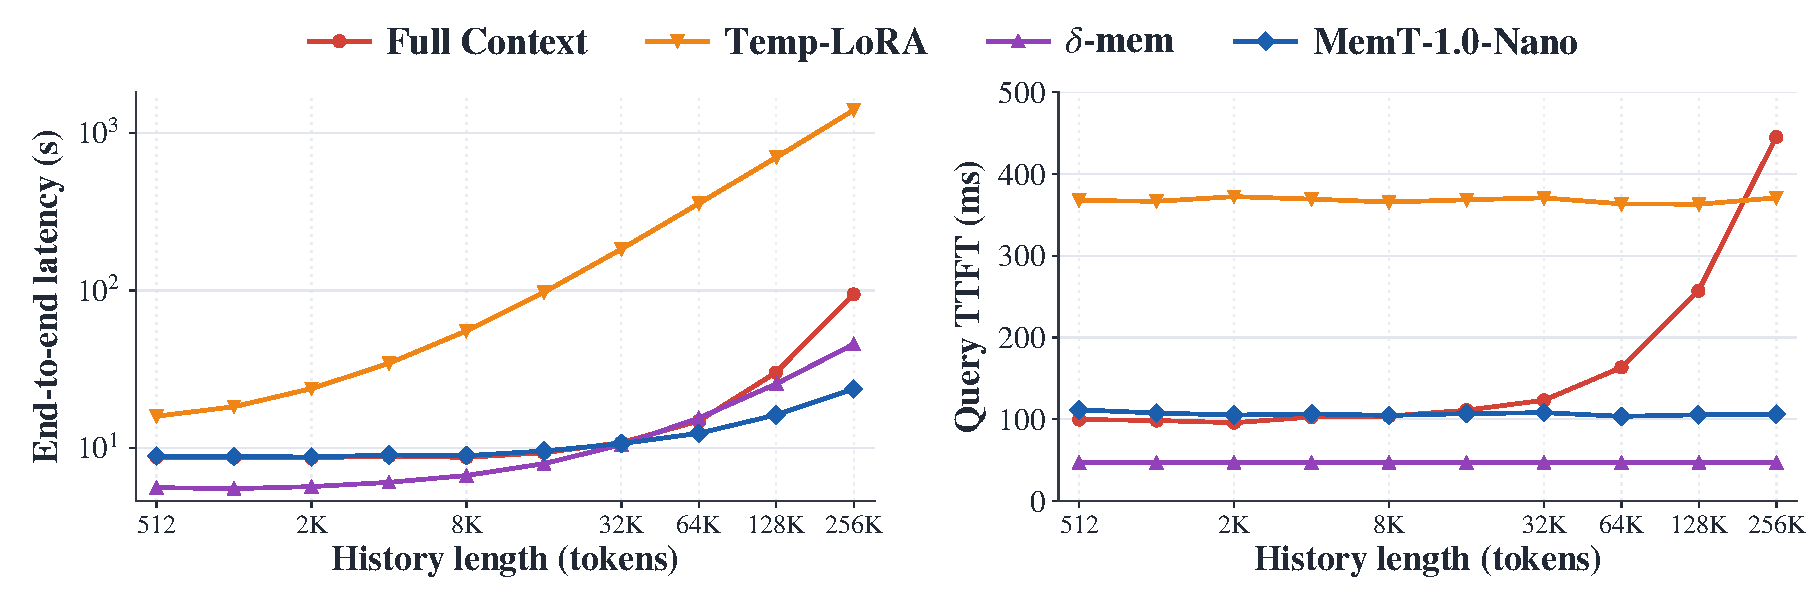
\includegraphics[width=\linewidth]{figures/eval_efficiency.pdf}
    \vspace{-0.8cm}
    \caption{Left: End-to-end latency includes history preparation and generation of a 128-token response. Right: Query TTFT measures the time from query execution to the first generated token, excluding history preparation.}
    \label{fig:results_efficiency}
    \vspace{-0.4cm}
\end{figure}

We construct input sequences with varying history lengths based on BEAM.
The query uses shared 512-token content, with the chat template added separately, rather than a benchmark question, and each sequence is treated independently.
We evaluate a fixed generation length of 128 tokens by forcing the model to decode exactly 128 tokens while ignoring the end-of-sequence signal.
For the HF evaluations, synchronized wall-clock timers exclude model loading, input tokenization, and evaluation-related scoring overhead.
For each history and length, we measure preparation once, discard one query warm-up, and average five timed queries. Reported curves average the resulting values across 35 histories.
For MemT-1.0-Nano, history content is processed in 2,048-token slices, with each chat-formatted chunk capped at 2,048 tokens.

The reported end-to-end latency includes history preparation and response generation, accounting for indexing, test-time adaptation, or memory writes as applicable.
We additionally report query time to first token (TTFT), measured from the start of query execution to the first generated token, including query prefilling but excluding history preparation.
For full context and MemT-1.0-Nano, both end-to-end latency and TTFT include state restoration.
The HF full-context baseline reuses the prepared history cache.
We report results over the common history-length range from 512 to 256K tokens.
Figure~\ref{fig:results_efficiency} presents the results.
MemT-1.0-Nano achieves an end-to-end advantage over full context at long histories.
It is generally slower at short histories and approximately matches full context at 32K tokens, reaching speedups of approximately $1.20\times$ at 64K, $1.86\times$ at 128K, and $3.99\times$ at 256K.
Its memory storage procedure processes history incrementally; generation then accesses the resulting state without retaining historical tokens in the attention context.
In comparison, the full-context baseline incurs both history prefilling and continued attention over historical KV entries during generation.
The measured long-history end-to-end advantage primarily reflects lower history-preparation cost.

The query TTFT curves reveal an additional benefit after history preparation.
MemT-1.0-Nano maintains broadly stable mean query TTFT of approximately 104--112\,ms across the evaluated range, while full-context TTFT rises to approximately 257\,ms at 128K tokens and 445\,ms at 256K tokens.
MemT-1.0-Nano's behavior is consistent with a fixed-size memory readout whose state dimensions do not grow with the number of historical tokens processed.
For persistent interactions, it allows accumulated history to influence responses without progressively increasing the attention context used for each new query.
The benefit concerns access to the stored representation, and the memory-capability results above already show that this representation preserves useful information.
At 128K and 256K tokens, MemT-1.0-Nano achieves query TTFT speedups of approximately $2.44\times$ and $4.19\times$, respectively, over cached full-context inference.

Previously collected results for the parametric memory baselines highlight the importance of accounting for preparation costs.
Temp-LoRA maintains stable query TTFT, but its end-to-end cost grows substantially because history-specific adaptation requires optimization.
Although $\delta$-mem has the lowest query TTFT, its end-to-end latency exceeds Nano's from 64K tokens onward as history-preparation cost grows.
Absolute latency differences across these systems also reflect their backbone, runtime, and tokenization configurations.
These results show the value of efficient memory construction together with predictable query TTFT.
Reusing a prepared state amortizes its construction cost over multiple queries.



\subsection{Storage Overhead}
\label{sec:storage_overhead}
We evaluate the per-trajectory storage overhead on BEAM histories, after history preparation and before querying.
The reported storage size is the logical size in bytes of the per-trajectory state.
The shared backbone weights, embedders and hyper memory parameters are excluded from the measurement.
More details can be found in Appendix~\ref{appendix:eval_storage_overhead}, and the results are presented in Figure~\ref{fig:storage_overhead}.

Figure~\ref{fig:storage_overhead} shows a clear difference between retaining historical records and maintaining a fixed-size state.
Full context incurs increasing storage as its logical state size grows with the visible history.
DenseRAG has a much smaller storage overhead at short histories, but its stored texts and retrieval vectors also accumulate as more information is added.
In contrast, MemT-1.0-Nano's memory state storage remains constant throughout the trajectory, because new information updates memory states without enlarging them.
At a history length of 128K tokens, MemT-1.0-Nano achieves an approximately $66\times$ reduction in per-trajectory storage compared with the full context setting.
Temp-LoRA also exhibits constant storage, since its adapter dimensions are fixed, although its storage overhead is larger than MemT-1.0-Nano's in the evaluated configuration.

The comparison with DenseRAG illustrates how the storage advantage depends on interaction length.
For short histories, storing a small collection of text chunks and embeddings is cheaper than allocating MemT-1.0-Nano's full memory state.
As histories grow, DenseRAG's accumulated records eventually exceed that fixed allocation.
MemT-1.0-Nano therefore becomes more attractive for persistent sessions with extended interaction histories, where additional turns do not increase the size of the saved state.
The full context curve ends at its context-window limit, so its reported storage does not represent retaining the entire longest history.
For deployment of MemT-1.0, a constant state size makes per-trajectory logical-state budgets predictable, and bounds the logical payload that must be saved or transferred when resuming an interaction.
Total storage still grows with the number of independent trajectories and the configured memory capacity.

\begin{figure}[t]
    \centering
    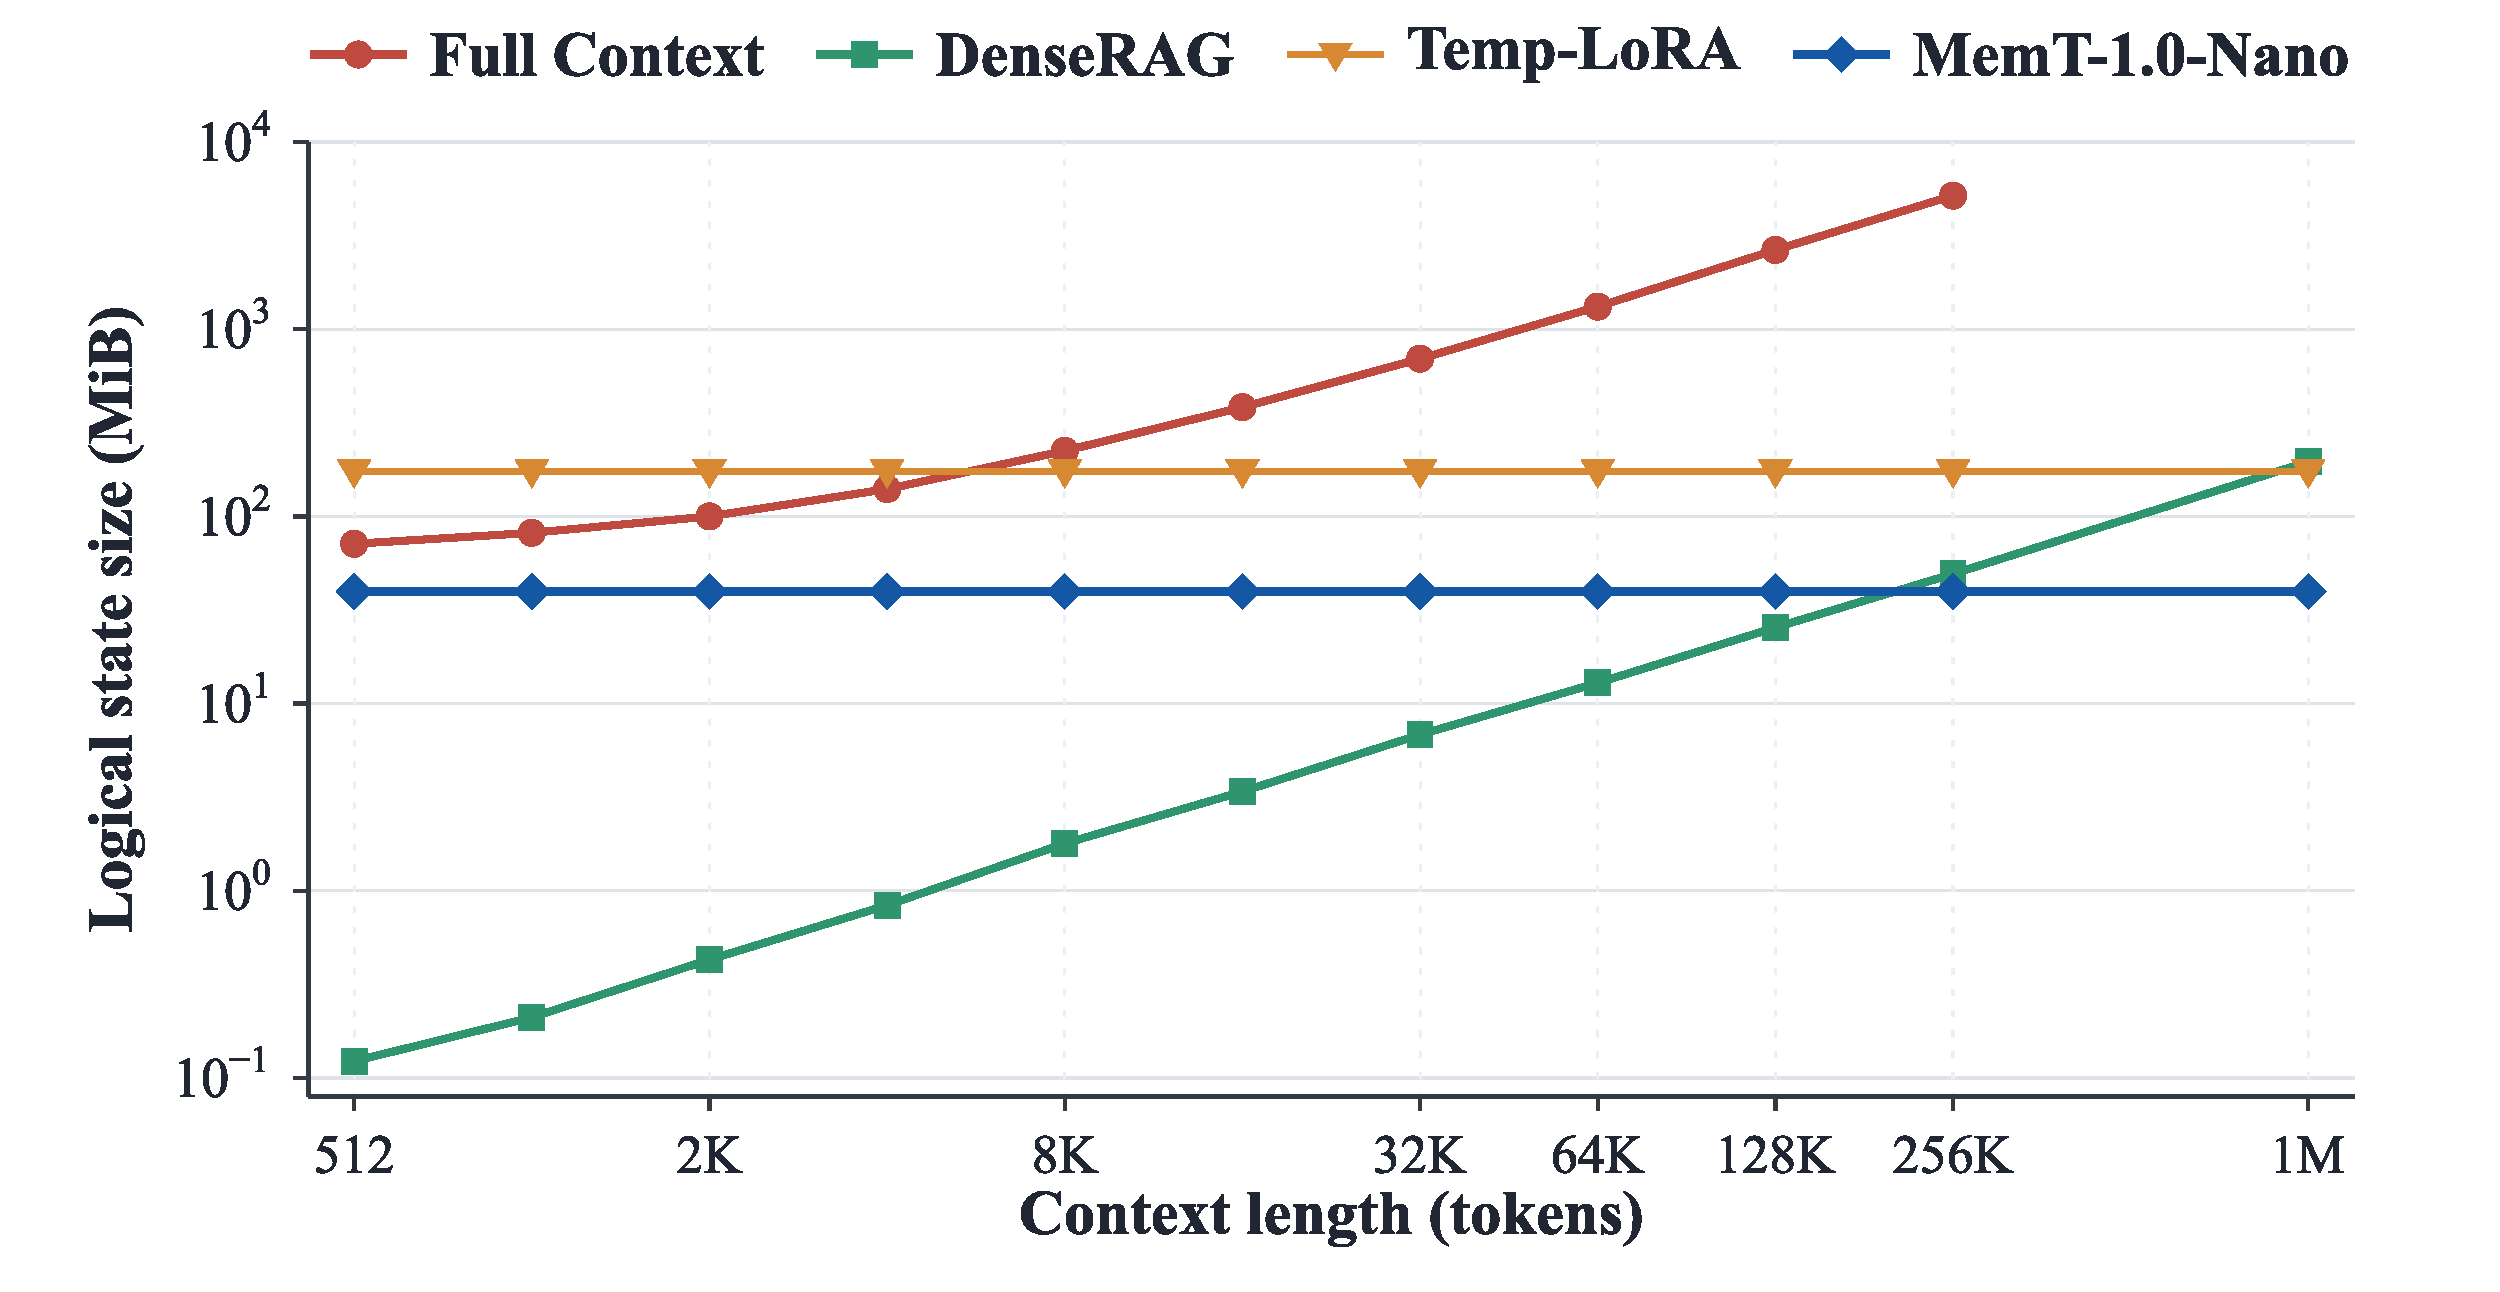
\includegraphics[width=0.75\linewidth]{figures/eval_storage.pdf}
    \vspace{-0.2cm}
    \caption{Results of storage overhead. Per-trajectory persistent storage on BEAM histories of increasing length.}
    \label{fig:storage_overhead}
    \vspace{-0.4cm}
\end{figure}


\subsection{Low-Rank Decomposition}
To further explore the compressibility of memory states based on MemT-1.0-Nano, we perform online low-rank projection for memory states to study their performance impacts.
Specifically, we apply singular value decomposition (SVD) to the FP32 state matrix of each layer after each storage procedure, and reconstruct a dense state from the retained components for subsequent computation.
For a retained rank $k$, the reconstructed state is computed as 
\begin{equation*}
    \mathbf{M}_{t,h}^{(l)}=U_{:,1:k}\Sigma_{1:k,1:k}V_{:,1:k}^{\top}.
\end{equation*}
We set the rank $k \in \{1, 2, 4, 8, 16, 32, 64, 128, 256\}$, with the full rank $k=256$ retaining the original dense state without projection.
The evaluation is conducted on PersonaMem and LoCoMo.
For each retention ratio, we independently initialize the memory state, write the complete history, and apply low-rank reconstruction after every memory storage  when $k<256$.

Figure~\ref{fig:low_rank_decomposition} shows different results across the two tasks.
On LoCoMo, accuracy generally improves as more singular components are retained.
The largest gains fall in the middle of the rank range, and the final doublings add progressively less, although the score still improves up to the full rank.
The one exception is the smallest retained rank, which scores slightly above the next one.
At this level of truncation, the small score difference alone does not establish an advantage of extreme compression.
PersonaMem follows the same shape but saturates much earlier.
Its accuracy rises quickly and then flattens out before reaching full rank, with the highest observed accuracy at an intermediate rank and no further improvement once additional components are retained.
Overall, memory performance improves as the retained rank increases, but the returns diminish quickly, and on PersonaMem they eventually vanish.
Because theoretical factor storage grows roughly linearly with the retained rank, increasing the rank yields diminishing returns in downstream accuracy.

\begin{figure}[t]
    \centering
    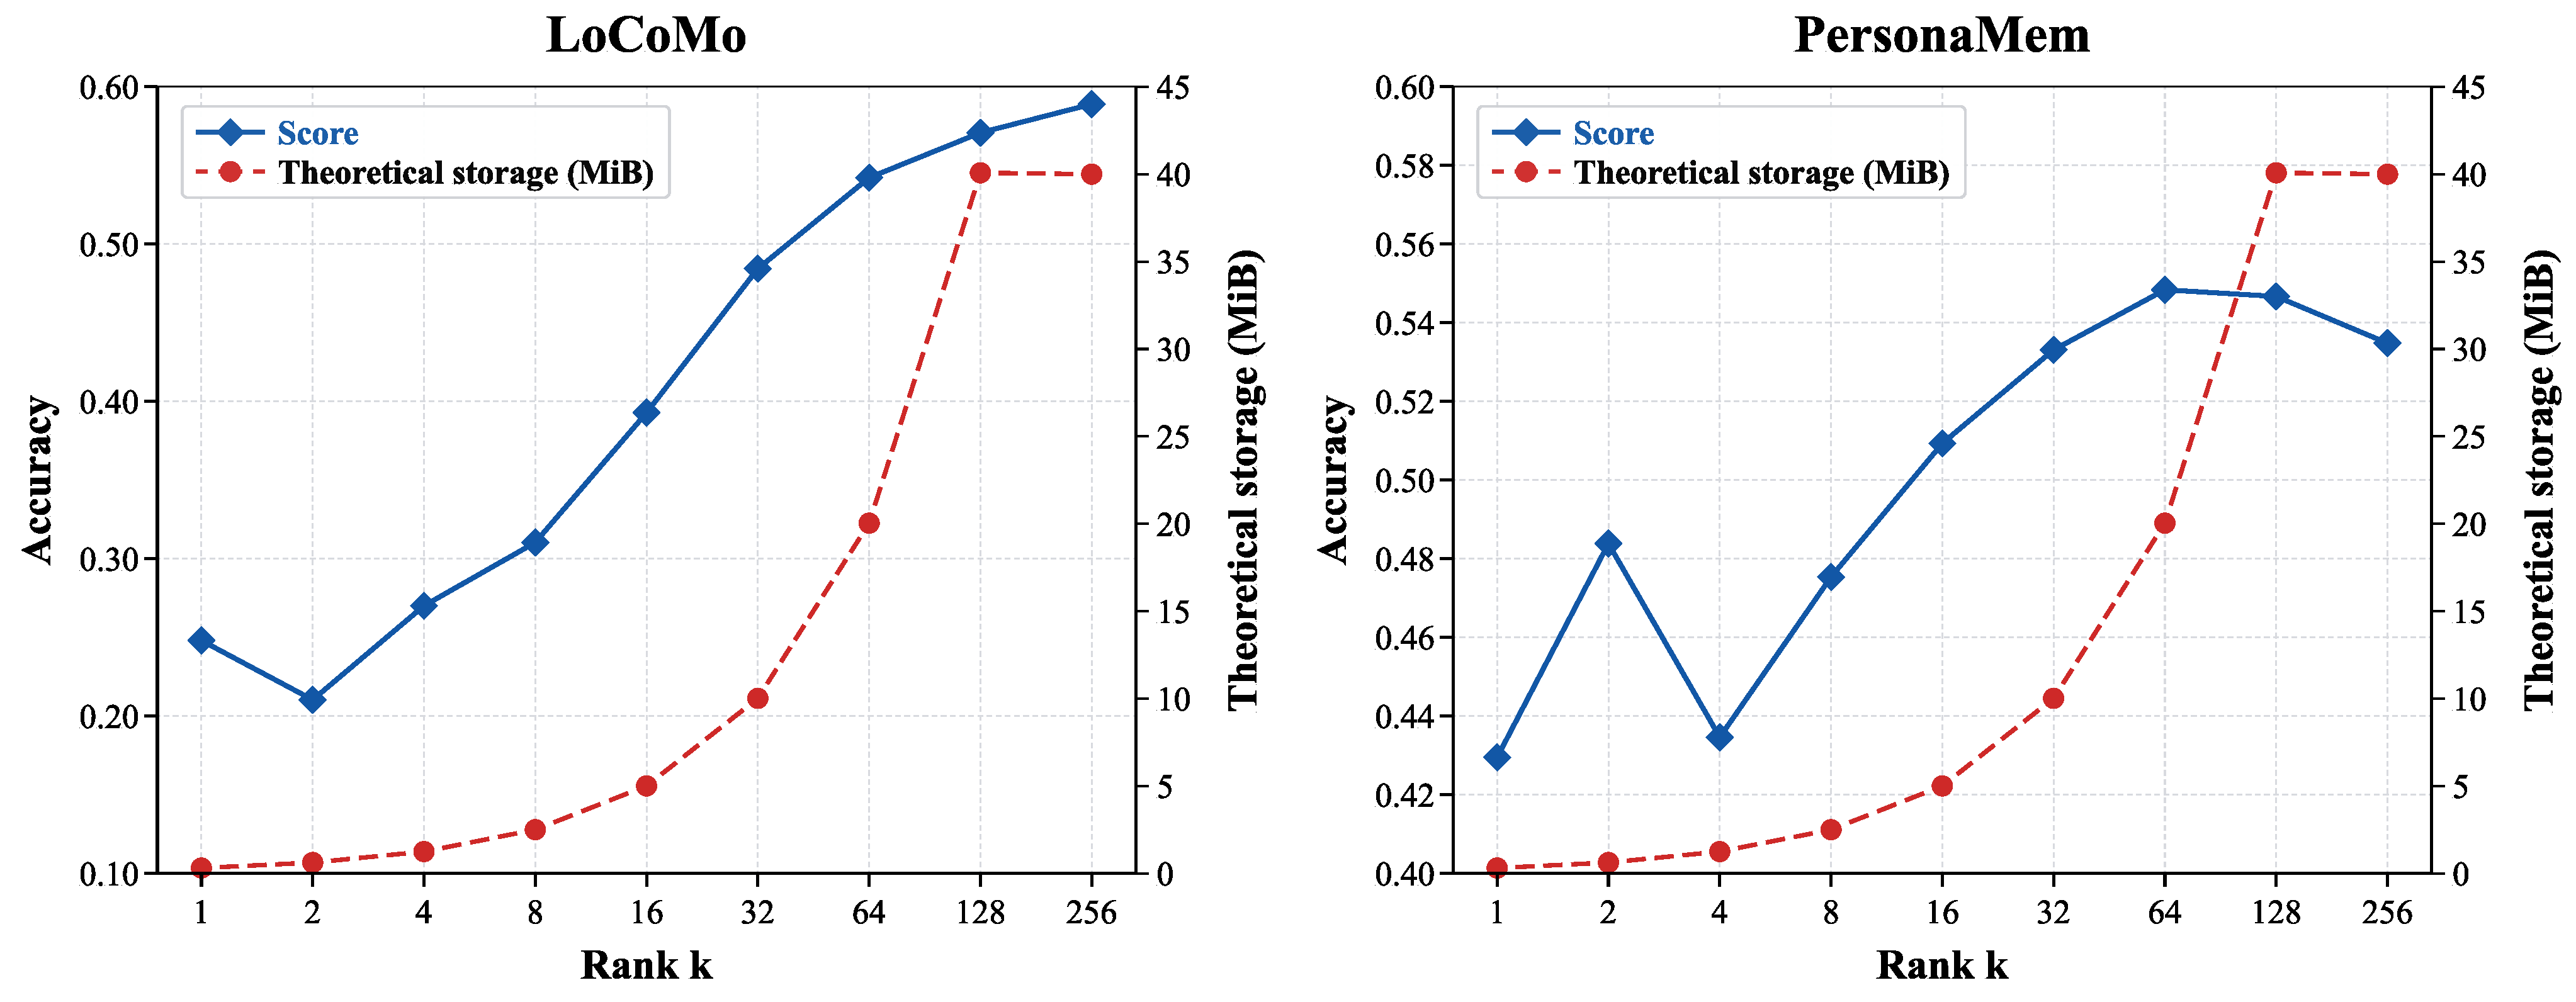
\includegraphics[width=0.95\linewidth]{figures/eval_low_rank.pdf}
    \vspace{-0.2cm}
    \caption{Impact of online low-rank decomposition
        on memory performance and storage.}
    \label{fig:low_rank_decomposition}
    \vspace{-0.4cm}
\end{figure}
